\subsection{Creation of \LaTeX\ Tutorials\\\LaTeX\ 教程的创建}\label{sec:latextutorial}

The following source code gives a guideline for the creation of \LaTeX\ tutorials.
In the next section, a framework for \LaTeX\ exercises is described.
All examples shall be numbered optionally.

以下源代码提供了创建 \LaTeX\ 教程的指南。 在下一节中,描述了 \LaTeX\ 练习的框架。 所有示例均可选择编号。

Firstly, some additional |tcb| keys are defined for the appearance.
For the examples, three environments |texexp|, |texexptitled|,
and |texexptitledspec| are defined with automatic numbering.

首先,为了外观方面定义了一些额外的 |tcb| 键。为了举例,定义了三个环境,即带自动编号的 |texexp|、|texexptitled| 和 |texexptitledspec|。
\begin{itemize}
\item |texexp| is used for untitled examples,
\\|texexp| 用于无标题的例子,
\item |texexptitled| is used for titled examples,
\\|texexptitled| 用于带标题的例子,
\item |texexptitledspec| is used for titled examples with special treatment.
\\|texexptitledspec| 用于带特殊处理的标题例子。
\end{itemize}

\inputpreamblelisting{D}

\begin{dispExample}
\begin{tcblisting}{texexp}
This is a \LaTeX\ example which displays the text as source code
and in compiled form.

这是一个展示文本源代码和编译后形式的 \LaTeX\ 示例。
\end{tcblisting}
\end{dispExample}


\begin{dispExample}
\begin{texexptitled}{First example with a title line}{firstExample}
Here, we use Example \ref{firstExample} with a title line.

在这里,我们使用带有标题行的示例\ref{firstExample}。
\end{texexptitled}
\end{dispExample}


\begin{dispExample}
\begin{texexp}{}
This is a \LaTeX\ example which displays the text as source code
and in compiled form.

这是一个 \LaTeX\ 的示例,它可以将文本显示为源代码和编译后的形式。
\end{texexp}
\end{dispExample}


\begin{dispExample}
\begin{texexp}{text and listing}
This is a \LaTeX\ example which displays the text as source code
and in compiled form.

这是一个 \LaTeX\ 的示例,它展示了文本的源代码和编译后的形式。
\end{texexp}
\end{dispExample}


\begin{dispExample}
\begin{texexp}{listing only}
This is a \LaTeX\ example which displays the text as source code only.

这是一个 \LaTeX\ 的例子,仅以源代码形式显示文本。
\end{texexp}
\end{dispExample}


\begin{dispExample}
\begin{texexp}{text only}
This is a \LaTeX\ example which displays the text in compiled form only.

这是一个 \LaTeX\ 示例,仅以编译后的形式展示文本。
\end{texexp}
\end{dispExample}


\begin{dispExample}
\begin{texexptitled}{An Example with a Heading}{heading1}
This is a \LaTeX\ example with a numbered heading line
which can be referred to.

这是一个带有编号标题行的 \LaTeX\ 示例,可以进行引用。
\end{texexptitled}
Here, we see Example \ref{heading1}.

在这里,我们看到示例\ref{heading1}。
\end{dispExample}


\begin{dispExample}
\begin{texexptitled}[listing only]{Another Example with a Heading}{heading2}
The keys can be used in combination. Here, an example with a heading line
and source code only is given.

这些键可以组合使用。下面是仅包含标题和源代码的示例。
\end{texexptitled}
Here, we see Example \ref{heading2}.

在这里,我们看到示例 \ref{heading2}。
\end{dispExample}


\begin{dispListing}
\begin{texexptitled}[float]{A floating Example with a Heading}{heading3}
This is another \LaTeX\ example with numbered heading line.
But now, the box is a floating object.

这是另一个带有编号标题行的 \LaTeX\ 示例。 但现在,这个框是一个浮动对象。
\end{texexptitled}
\end{dispListing}
\tcbusetemp

\begin{dispExample}
The floating box of the last example is seen as Example \ref{heading3}
on page \pageref{heading3}.

上一个例子中的浮动框在第\pageref{heading3}页被视为第\ref{heading3}个例子。
\end{dispExample}


\begin{dispExample}
\begin{texexptitledspec}{Special application}{texexpbox1}
\begin{lstlisting}[style=tcblatex]
Some \LaTeX\ source code.

一些 \LaTeX\ 源代码。
\end{lstlisting}
\tcblower
For special cases, the environment |texexptitledspec| with style
|example| can be used directly. As one can see, the upper and the lower
part of the box can be used uncoupled also.

对于特殊情况,可以直接使用样式为|example|的环境|texexptitledspec|。可以看到,盒子的上部和下部也可以分开使用。
\end{texexptitledspec}
\end{dispExample}


The following series of examples demonstrate the application of
\refEnvLe{tcolorbox} options for diversification.

以下一系列例子展示了 \refEnvLe{tcolorbox} 选项的多样化应用。
\begin{dispExample}
\begin{texexptitled}{How to use options (1):\par The basic example}{options1}
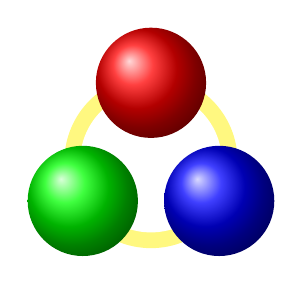
\begin{tikzpicture}
\path[fill=yellow!50!white] (0,0) circle (11mm);
\path[fill=white] (0,0) circle (9mm);
\foreach \w/\c in {90/red,210/green,330/blue}
{\path[shading=ball,ball color=\c] (\w:1cm) circle (7mm);}
\end{tikzpicture}
\end{texexptitled}
\end{dispExample}


\begin{dispExample}
\begin{texexptitled}[center lower,enhanced,segmentation hidden,middle=0mm]
{How to use options (2):\par The text output is centered and the
segmentation line has vanished.}{options2}
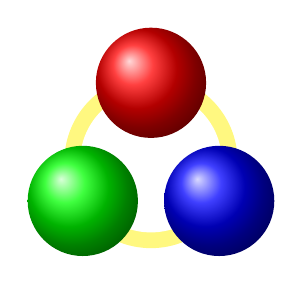
\begin{tikzpicture}
\path[fill=yellow!50!white] (0,0) circle (11mm);
\path[fill=white] (0,0) circle (9mm);
\foreach \w/\c in {90/red,210/green,330/blue}
{\path[shading=ball,ball color=\c] (\w:1cm) circle (7mm);}
\end{tikzpicture}
\end{texexptitled}
\end{dispExample}

\begin{dispExample}
\begin{texexptitled}[tikz lower,bicolor,colbacklower=white]
{How to use options (3):\par Here, the |tikzpicture| is totally hidden.
The |bicolor| skin highlights the output.}{options3}
\path[fill=yellow!50!white] (0,0) circle (11mm);
\path[fill=white] (0,0) circle (9mm);
\foreach \w/\c in {90/red,210/green,330/blue}
{\path[shading=ball,ball color=\c] (\w:1cm) circle (7mm);}
\end{texexptitled}
\end{dispExample}

\begin{dispExample}
\begin{texexptitled}[center lower,listing side text,righthand width=3.5cm,
bicolor,colbacklower=white]
{How to use options (4):\par The |bicolor| skin also works with side
by side mode}{options4}
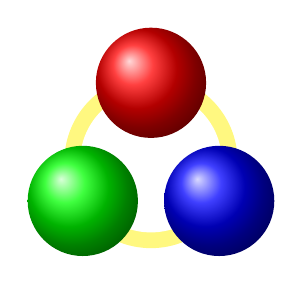
\begin{tikzpicture}
\path[fill=yellow!50!white] (0,0) circle (11mm);
\path[fill=white] (0,0) circle (9mm);
\foreach \w/\c in {90/red,210/green,330/blue}
{\path[shading=ball,ball color=\c]
(\w:1cm) circle (7mm);}
\end{tikzpicture}
\end{texexptitled}
\end{dispExample}


\begin{dispExample}
\begin{texexptitled}[center lower,listing outside text,righthand width=3.5cm]
{How to use options (5):\par Putting our picture outside is just
a matter of one word.}{options5}
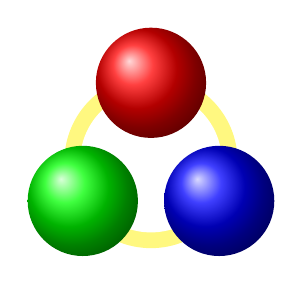
\begin{tikzpicture}
\path[fill=yellow!50!white] (0,0) circle (11mm);
\path[fill=white] (0,0) circle (9mm);
\foreach \w/\c in {90/red,210/green,330/blue}
{\path[shading=ball,ball color=\c]
(\w:1cm) circle (7mm);}
\end{tikzpicture}
\end{texexptitled}
\end{dispExample}


\begin{dispExample}
\begin{texexptitled}[center lower,text above listing]
{How to use options (6):\par The picture may also be put above
the listing box.}{options6}
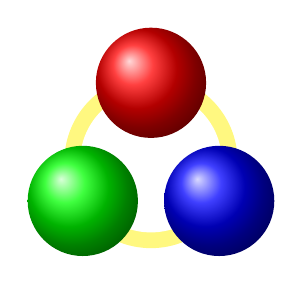
\begin{tikzpicture}
\path[fill=yellow!50!white] (0,0) circle (11mm);
\path[fill=white] (0,0) circle (9mm);
\foreach \w/\c in {90/red,210/green,330/blue}
{\path[shading=ball,ball color=\c]
(\w:1cm) circle (7mm);}
\end{tikzpicture}
\end{texexptitled}
\end{dispExample}


\begin{dispExample}
\begin{texexptitled}[beamer,center lower,text outside listing,lefthand width=3.5cm]
{How to use options (7):\par Our style is easily transformed into
a beamerish one.}{options7}
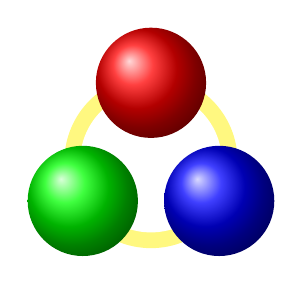
\begin{tikzpicture}
\path[fill=yellow!50!white] (0,0) circle (11mm);
\path[fill=white] (0,0) circle (9mm);
\foreach \w/\c in {90/red,210/green,330/blue}
{\path[shading=ball,ball color=\c]
(\w:1cm) circle (7mm);}
\end{tikzpicture}
\end{texexptitled}
\end{dispExample}